%%=============================================================================
%% Methodologie
%%=============================================================================

\chapter{Methodologie}
\label{ch:methodologie}
\lstset{
    tabsize = 4, %% Sets tab space width.
    showstringspaces = false, %% Prevents space marking in strings, string is defined as the text that is generally printed directly to the console.
    numbers = left, %% Displays line numbers on the left.
    commentstyle = \color{green}, %% Sets comment color.
    keywordstyle = \color{blue}, %% Sets  keyword color.
    stringstyle = \color{red}, %% Sets  string color.
    rulecolor = \color{black}, %% Sets frame color to avoid being affected by text color.
    basicstyle = \small \ttfamily , %% Sets listing font and size.
    breaklines = true, %% Enables line breaking.
    numberstyle = \tiny,
}

%%\begin{lstlisting}[language = Java , frame = trBL , firstnumber = last , escapeinside={(*@}{@*)}]
%%public class Factorial
%%{
%%public static void main(String[] args)
%%{   final int NUM_FACTS = 100;
%%for(int i = 0; i < NUM_FACTS; i++)
%%System.out.println( i + "! is " + factorial(i));
%%}
%%
%%public static int factorial(int n)
%%{   int result = 1;
%%for(int i = 2; i <= n; i++) (*@\label{for}@*)
%%result *= i;
%%return result;
%%}
%%}
%%\end{lstlisting}


%% TODO: Hoe ben je te werk gegaan? Verdeel je onderzoek in grote fasen, en
%% licht in elke fase toe welke stappen je gevolgd hebt. Verantwoord waarom je
%% op deze manier te werk gegaan bent. Je moet kunnen aantonen dat je de best
%% mogelijke manier toegepast hebt om een antwoord te vinden op de
%% onderzoeksvraag.

% TODO: uitleg wat we allemaal nodig hebben, producer uitleggen, consumer uitleggen, 3 verschillende groottes uitleggen.
Om te testen welke van de technologieën die in dit onderzoek aan bod komen nu eigenlijk het beste is, zou je met veel zaken rekening moeten houden. Wat het beste is hangt namelijk af van welke soort data je gebruikt. Ook de hoeveelheid transformaties die je data ondergaan voor dat het uitgelezen wordt of verzonden speelt een grote rol. Natuurlijk is het moeilijk om binnen de tijdspanne die er is voor dit onderzoek al deze factoren te gaan onderzoeken. Daarom zal dit onderzoek zich toespitsen op een bepaald scenario en daar conclusies uit trekken.  
\section{Producer project}
Het opzetten van een omgeving is per technologie verschillend. Elk heeft zijn eigen manier om data te verzenden en te ontvangen. Hieronder wordt eerst eens per technologie de implementatie getoond hoe we het project opgezet hebben. Daarna wordt er uitgelegd hoe we gaan testen welke nu de beste zal zijn. De reden waarom we specifiek deze technologieën gekozen hebben om te vergelijken kan opnieuw gelezen worden in de Stand van Zaken en de Inleiding.  

Natuurlijk moet er iets gelijkaardigs zijn om te kunnen vergelijken. Het data object dat we zullen verzenden en ontvangen bij zowel \emph{Kafka}, \emph{RabbitMq} en \emph{Google Pub/Sub} zal hetzelfde zijn. Op deze manier is het toekomstige resultaat niet afhankelijk van het type data. Dit onderzoek zal zich dus toespitsen op data met het type Json. Deze klasse (Data.class) hergebruiken we in elke technologie. Deze klasse is het type van het bericht dat we verzenden.
\begin{lstlisting}[language = Java , frame = trBL , firstnumber = last , escapeinside={(*@}{@*)}]
@Getter
@AllArgsConstructor
@NoArgsConstructor
@ToString
public class Data {
    private int id;
    private String name;
    private String description;
    private Date sendedDate;
}
     \end{lstlisting}
     
Deze klasse bevat vier attributen. Dit is om een Json object na te bootsen. Het is vanzelfsprekend dat deze klasse niet zo maar automatisch kan omgezet worden naar een Json. De manier waarop dit gedaan wordt is opnieuw per technologie verschillend. De uitleg zal gegeven worden in de subsectie van de technologie zelf hoe het omzetten gebeurd. De attributen die hier gebruikt worden zijn: een id van het type int, dit is om elk data object van elkaar te kunnen onderscheiden tijdens het verzenden. Als tweede zie je naam van het type String. Dit heeft als bedoeling opnieuw om verschillende objecten van elkaar te kunnen onderscheiden en om een realistische attribuut te geven aan het Data-object. Deze reden is hetzelfde voor het attribuut description van het type String. Als laatste hebben we de sendedDate van het type Date. Deze zal de datum en het tijdstip doorsturen van het moment wanneer het object verzonden is. Dit zal later nog eens aangehaald worden wanneer we deze objecten genereren. 

Als u boven de klasse kijkt dan ziet u nog vier annotaties staan. Deze kunnen we gebruiken door de library van lombok. Dit werd mogelijk gemaakt door deze dependency toe te voegen aan onze pom.xml want het gebruikte project voor dit onderzoek maakt gebruik van Maven om libraries toe te voegen.

\begin{lstlisting}[language = xml , frame = trBL , firstnumber = 1 , escapeinside={(*@}{@*)}]
<dependency>
<groupId>org.projectlombok</groupId>
<artifactId>lombok</artifactId>
<optional>true</optional>
</dependency>
\end{lstlisting}

Deze geeft op voorhand al enkele handige implementaties. De gebruikte annotaties zullen we uitleggen, want natuurlijk bestaan er meer dan enkel deze die dit onderzoek gebruikt. Voor de andere mogelijkheden verwijs ik u graag door naar de site van Project Lombok waar u alle mogelijkheden op een rijtje ziet: https://projectlombok.org/features/all. 

De eerste annotatie is @Getter, deze zorgt ervoor zoals de naam al doet vermoeden, dat er voor ieder attribuut een getter aanwezig is. Op deze manier staat uw code niet overvol met getters van al uw attributen. In deze klasse zijn er niet zo veel attributen dus zou het aantal getter nog meevallen. Maar u kan zich wel inbeelden dat in een groter project in een klasse met veel attributen en andere methodes dat dit een handige annotatie is. Je ziet dus niet dat de getters aanwezig zijn maar die zijn er wel effectief. Laten we de tweede en de derde samen bekijken: @AllArgsConstructor en @NoArgsConstructor. Deze zorgen ervoor dat er een constructor gegenereerd wordt met respectievelijk al de attributen en zonder de attributen. Deze zijn vaak voorkomende constructors en zijn handig om ook hiervoor een annotatie te hebben. De laatste  is de @ToString. Deze werd gebruikt tijdens de opmaak van het project. Dit vormt het object om in een String. Dit was handig om lokaal te testen. Het data object werd dan uitgeprint tijdens het verzenden om te controleren als het object wel de juiste waardes bevatte.
\subsection{Kafka}
In figuur 3.1 ziet u welke configuratie de topic heeft. Er wordt gebruik gemaakt van zes partities en de data wordt vier weken bijgehouden. Met andere woorden: als de data op de topic komt, en deze niet binnen de vier weken door een consumer, dan wordt de data verwijderd en kan deze data niet meer opnieuw uitgelezen worden.
\begin{figure}[h!]
    \centering
    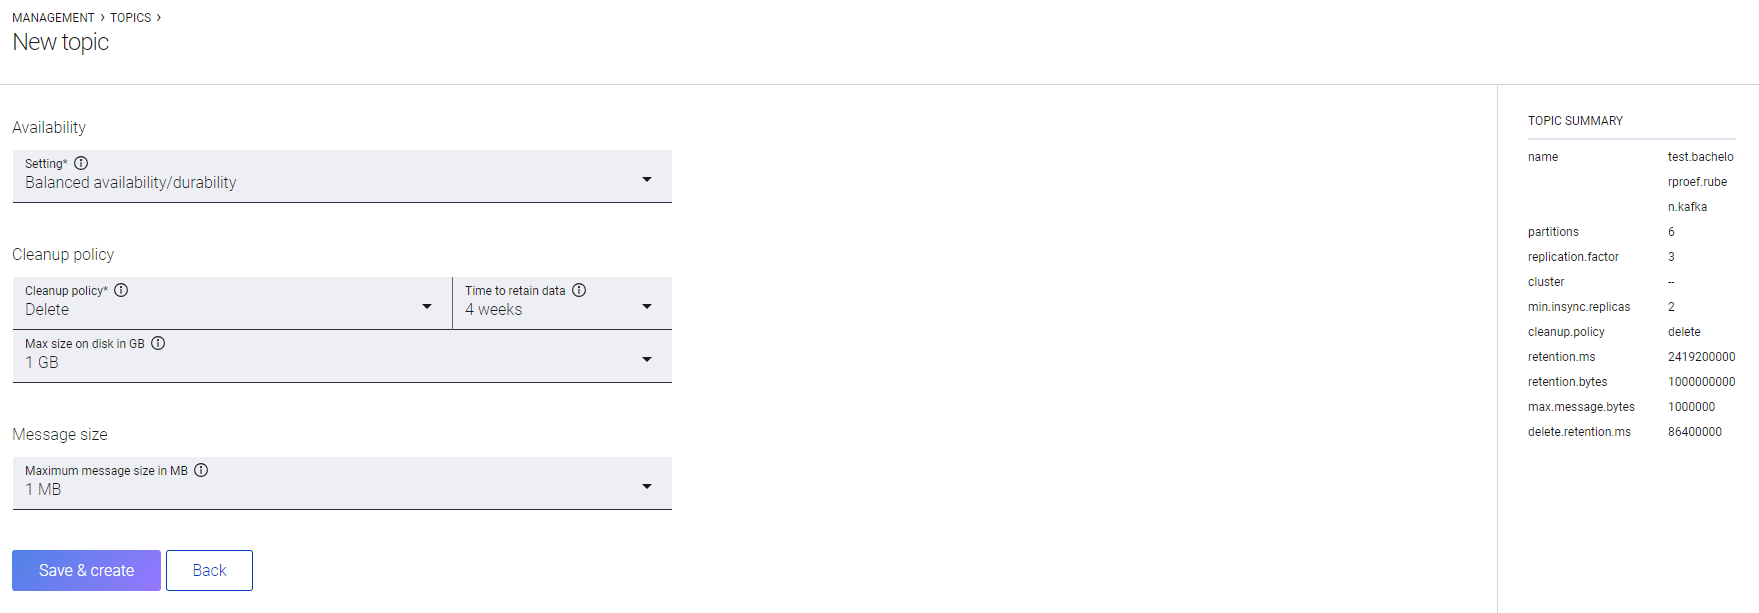
\includegraphics[width=140mm]{../kafkaConfig.png}
    \caption{Configuratie van de topic}
    
\end{figure}
\subsubsection{KafkaConfig}
Zo ziet de implementatie van de KafkaConfig.class eruit.

    \begin{lstlisting}[language = Java , frame = trBL , firstnumber = 1 , escapeinside={(*@}{@*)}]
    @Configuration
    public class KafkaConfig {
        
        @Bean
        @Primary
        public KafkaProperties kafkaProperties(
        @Value("${kafka_key}") final String kafkaKey,
        @Value("${kafka_secret}") final String kafkaSecret
        
        ) {
            KafkaProperties kafkaProperties = new KafkaProperties();
            
            KafkaProperties.Producer producer = kafkaProperties.getProducer();
            
            producer.getProperties().put(ProducerConfig.KEY_SERIALIZER_CLASS_CONFIG, "org.apache.kafka.common.serialization.StringSerializer");
            producer.getProperties().put(ProducerConfig.VALUE_SERIALIZER_CLASS_CONFIG, "org.springframework.kafka.support.serializer.JsonSerializer");
            
            producer.getProperties().put(ProducerConfig.BOOTSTRAP_SERVERS_CONFIG, "pkc-412nj.europe-west1.gcp.confluent.cloud:9092");
            producer.getProperties().put(ProducerConfig.RETRIES_CONFIG, "0");
            producer.getProperties().put(ProducerConfig.ACKS_CONFIG, "all");
            producer.getProperties().put(ProducerConfig.RETRY_BACKOFF_MS_CONFIG, "1000");
            producer.getProperties().put(ProducerConfig.REQUEST_TIMEOUT_MS_CONFIG, "30000");
            producer.getProperties().put(ProducerConfig.LINGER_MS_CONFIG, "200");
            kafkaProperties.getProperties().put(SslConfigs.SSL_ENDPOINT_IDENTIFICATION_ALGORITHM_CONFIG, "https");
            kafkaProperties.getProperties().put(SaslConfigs.SASL_MECHANISM, "PLAIN");
            kafkaProperties.getProperties().put("request.timeout.ms", "20000");
            kafkaProperties.getProperties().put("retry.backoff.ms", "500");
            kafkaProperties.getProperties().put(SaslConfigs.SASL_JAAS_CONFIG, "org.apache.kafka.common.security.plain.PlainLoginModule required username=\""
            + kafkaKey + "\" password=\"" + kafkaSecret + "\";");
            kafkaProperties.getProperties().put("security.protocol", "SASL_SSL");
            
            kafkaProperties.getProperties().put(JsonSerializer.ADD_TYPE_INFO_HEADERS, "false");
            
            return kafkaProperties;
        }
            \end{lstlisting}
            
     In deze klasse ziet u dat het instellen van de nodige properties in de kafkaProperties methode van deze klasse gebeurd. Deze zouden ook in de application.yml file kunnen ingesteld worden. In dit project van het onderzoek hebben we besloten om dit in een config klasse te doen. Tijdens het opzetten van het project kon de applicatie de properties niet uitlezen vanuit de application.yml file. Om geen tijd te verliezen hebben we besloten om deze properties in een config klasse in te stellen. Dit verandert niets van functionaliteit of aan resultaten van dit onderzoek. Maar als onderzoeker was het mogelijk om sneller aan de slag te gaan met het belangrijkere werk.
     
     Boven de klasse ziet u de annotatie @Configuration. Dit is een annotatie van het Spring framework. Deze zorgt ervoor dat je aangeeft dat deze klasse een configuratie instelt. In de klasse ziet u boven de methode kafkaProperties twee andere annotaties staan. @Bean zorgt ervoor dat er een bean aangemaakt wordt voor deze methode. Dit zorgt ervoor dat door het Spring framework voor deze methode eerder een instantie aangemaakt wordt en daardoor de applicatie bij het opstarten deze properties kan instellen. Daaronder zie je een andere annotatie die hiermee te maken heeft: @Primary. Deze zorgt ervoor als het Spring framework meerdere beans heeft van KafkaProperties, dat hij deze voorneemt op al de andere. Op deze manier zijn we zeker dat deze properties gebruikt worden en niet andere indien er meerdere beans zouden zijn.
     
     U ziet dat er tamelijk wat properties geconfigureerd zijn. Er zullen slechts enkele properties besproken worden, uiteraard zijn dit de belangrijkste voor dit onderzoek. In dit hoofdstuk werd al eens vermeld dat het object van de klasse Data niet zomaar omgezet wordt naar een Json. Hiervoor is er een serializer nodig die dit doet. Op lijn 16 van de KafkaConfig klasse is er te zien dat de gekozen serializer ingesteld wordt. In dit geval wordt de JsonSerializer gebruikt uit de package springframework.kafka.support.serializer. Dit is dus een specifieke JsonSerializer voor Kafka. De key wordt dan weer geserializeerd naar een String door de StringSerializer uit de package org.apache.kafka.common.serialization, dit is te zien op de regel er boven. Wat als het niet lukt voor de producer om de data te verzenden? In ons geval mag hij dit niet opnieuw proberen. Op deze manier kunnen we ook te weten komen hoeveel data er mislukt is om te verzenden. Dit zie je op lijn 19. Indien je meer zekerheid wilt dat je een data object zeker verzonden wordt, dan kan je deze property in plaats van 0 op bijvoorbeeld 3 zetten. Je mag zeker ook niet vergeten om de username en password mee te geven van waar je Kafka topic zich bevindt. Op lijn 28 en 29 zie je dat dit meegegeven wordt. De username en wachtwoord worden niet in plaintext in de code geplaatst. Het is niet de bedoeling dat iedereen weet wat het wachtwoord en username is. Deze worden ingesteld in uw application.yml en worden meegegeven via de parameters van de methode door het spring framework. Door de annotatie @Value en de naam van de key van uw waarden in de application.yml, weet spring perfect waar hij het wachtwoord en username moet gaan halen.
     
    \subsubsection{KafkaPublisher}
    De KafkaPublisher.class is de effectieve producer van Data objecten. Veel moet er niet ingesteld worden om deze producer te doen laten werken. Wat je zeker moet hebben is een KafkaTemplate en de naam van de topic waarnaar je verzend. Laat ons even deze klasse stap voor stap bekijken.
    
    Boven de klasse staat de annotatie @Component. Dit is opnieuw een annotatie van het spring framework. Deze zorgt ervoor dat je via constructor- of setterinjectie in andere klasses telkens dezelfde instantie van de klasse KafkaPublisher kunt gebruiken. Op die manier moet je niet telkens een nieuwe instantie maken van de klasse. Er zijn twee attributen: de kafkaTemplate van het type KafkaTemplate en een String topicName; De KafkaTemplate is een template die je gebruikt om je message naar een Kafka topic te verzenden.
    
    In de constructor worden kafkaTemplate en topicName meegegeven als parameters. Spring Boot zorgt ervoor dat de kafkaTemplate automatisch gecreëerd wordt. De topicName willen we niet zo maar in onze code schrijven, dus injecteren we die vanuit de application.yml. Hiervoor wordt opnieuw @Value gebruikt, maar dit principe werd al eens uitgelegd.
    
    Als laatste bevat deze klasse ook nog de publish methode. Deze verzend een message effectief naar de topic. In onze implementatie krijgt deze methode een lijst van Data objecten mee. In dit onderzoek is het niet van toepassing om één enkel Data object te verzenden, dus om praktische redenen wordt er een lijst meegegeven. In deze methode wordt deze lijst overlopen en telkens worden dezelfde operaties uitgevoerd. Er wordt een object aangemaakt van de klasse Message, zoals de naam al doet vermoeden wordt dit onze message. In de payload van deze message stoppen we ons Data object. In de header geven we twee zaken mee. Als message key geven we het id mee, omdat in deze implementatie het id toch telkens uniek zal zijn. Als tweede moeten we nog de naam van onze topic meegeven zodat de kafkaTemplate weet naar waar hij moet versturen. Het enigste dat deze methode dan nog moet doen is de kafkaTemplate gebruiken om de message te verzenden. Het omzetten van de message in een json formaat wordt automatisch gedaan omdat we in de properties een serializer opgegeven hebben. Ook de message key wordt voor dezelfde reden automatisch geserializeerd. 
 
        \begin{lstlisting}[language = Java , frame = trBL , firstnumber = 1 , escapeinside={(*@}{@*)}]
    @Component
    public class KafkaPublisher {
        
        private KafkaTemplate kafkaTemplate;
        private String topicName;
        
        public KafkaPublisher(KafkaTemplate kafkaTemplate,
        @Value("${kafka.topic.name}") String topicName) {
            this.kafkaTemplate = kafkaTemplate;
            this.topicName = topicName;
        }
        
        public void publish(List<Data> dataList) {
            for (Data data : dataList) {
                Message<Data> message = MessageBuilder.withPayload(data)
                .setHeader(KafkaHeaders.MESSAGE_KEY, String.valueOf(data.getId()))
                .setHeader(KafkaHeaders.TOPIC, topicName)
                .build();
                
                kafkaTemplate.send(message);
            }
        }
    }
     \end{lstlisting}
\subsection{RabbitMq}
\subsubsection{RabbitMqConfig}
In dit onderzoek zijn alle configuraties van RabbitMq gedaan in application.yml. 
        \begin{lstlisting}[language = xml , frame = trBL , firstnumber = 1 , escapeinside={(*@}{@*)}]
spring:
    rabbitmq:
        host: "hostadress"
        port: 16379
        username: ${rabbitmq_username}
        password: ${rabbitmq_password}
        virtual-host: "rabbitmq"
        ssl:
            enabled: true
            algorithm: "TLSv1.2"
        listener:
         simple:
            default-requeue-rejected: false
        direct:
            default-requeue-rejected: false
     \end{lstlisting}
     
     Veel configuraties zijn er niet. De belangrijkste zijn host, port, username en password. De host is het adres waar uw RabbitMq exchange op draait met de juiste poort die opgegeven wordt in port. In het project is de String ''hostadress'' vervangen door de effectieve host. Om privacy redenen is hier dit adres gewijzigd. Username en password worden ook nog bijgehouden in een variabele maar deze staan natuurlijk niet op het codevoorbeeld. Hiernaast wordt ook nog de naam van de exchange bijgehouden die we later in de implementatie nodig zullen hebben. Uiteraard zit deze property ook niet in het codevoorbeeld.
     
 \subsubsection{RabbitMqPublisher}
 Over het algemeen gezien kun je deze klasse goed vergelijken met de KafkaPublisher klasse. Het grootste verschil zit men in de publish methode. De annotatie @Component boven de klasse heeft hetzelfde doel als bij de KafkaPublisher. Er is hier één attribuut meer en dat is de ObjectMapper. Deze wordt gebruikt om later in de publish methode onze data om te zetten naar een String. Uiteraard is de KafkaTemplate hier vervangen door een RabbitTemplate. Deze hebben dezelfde functionaliteit maar bij een verschillende technologie. Het is dus ook een template die je gebruikt om de data te verzenden naar de exchange. Hier heb je niet de naam van de topic nodig zoals bij de KafkaPublisher maar de naam van de exchange.
 
 In de constructor wordt de rabbitTemplate en de objectMapper opnieuw automatisch gecreëerd door Spring Boot. De naam van de exchange wordt weer via de application.yml file geïnjecteerd. In de publish methode overlopen we weer een lijst van objecten van Data. Bij iedere elementje uit de lijst voeren we dezelfde operaties uit. We gebruiken de objectMapper om ons object om te zetten naar een String. Het resultaat van deze String is in een Json formaat. Dit kunnen we ook verifiëren en daarom is als laatste lijn in de for-lus een print-statement toegevoegd. Deze String wordt uitgeprint en we kunnen mooi zien dat deze String een Json formaat heeft. Verder gebruiken we de rabbitTemplate om ons bericht te verzenden naar de exchange die we meegeven samen met ons bericht.
   \begin{lstlisting}[language = java , frame = trBL , firstnumber = 1 , escapeinside={(*@}{@*)}]
 @Component
 public class RabbitMqPublisher {
     private RabbitTemplate rabbitTemplate;
     private ObjectMapper objectMapper;
     private String exchangeName;
     
     public RabbitMqPublisher(final RabbitTemplate rabbitTemplate,
     final ObjectMapper objectMapper,
     @Value("${rabbitmq.topic.exchange.name}") final String exchangeName) {
         this.rabbitTemplate = rabbitTemplate;
         this.objectMapper = objectMapper;
         this.exchangeName = exchangeName;
     }
     
     public void publish(final List<Data> dataList) {
         try {
             for (Data data : dataList) {
                 String stringData = objectMapper.writeValueAsString(data);
                 
                 rabbitTemplate.convertAndSend(exchangeName, "", stringData);
                 System.out.println("sending messeage RMQ: " + stringData);
             }
             
         } catch (JsonProcessingException e) {
             e.printStackTrace();
         }
     }
 }
     \end{lstlisting}
\subsection{Google Pub/Sub}
Op figuur 3.2 kunt u zien hoe de configuratie van de topic is voor de gebruikte subscription in dit onderzoek. We zien dat bij het lezen van een message die op de Pub/Sub staat, dat er een tijdlimiet staat van 60 seconden. Dit wil zeggen dat indien de message binnen de 60 seconden niet gelezen kan worden wanneer de subscriber messages aan het lezen is, dat de actie NACK uitgevoerd wordt op deze message. Dit wil zeggen dat de message nog altijd niet verwijderd is van de topic en dat deze nog altijd gelezen kan worden door de subscriber. Bij Google Pub/Sub kun je deze tijdslimiet instellen tussen 60 en 600 seconden. Onder de ''Acknowledgement''' Deadline ziet u ''Message retention duration'' staan. Dit is hoe lang een message op de topic blijft staan. In dit geval staat deze waarde op het maximum: op zeven dagen. Met andere woorden: indien een message binnen de zeven dagen niet gelezen wordt, dan zal deze verwijderd worden en is het niet meer mogelijk om deze message terug te vinden.
\begin{figure}[h!]
    \centering
    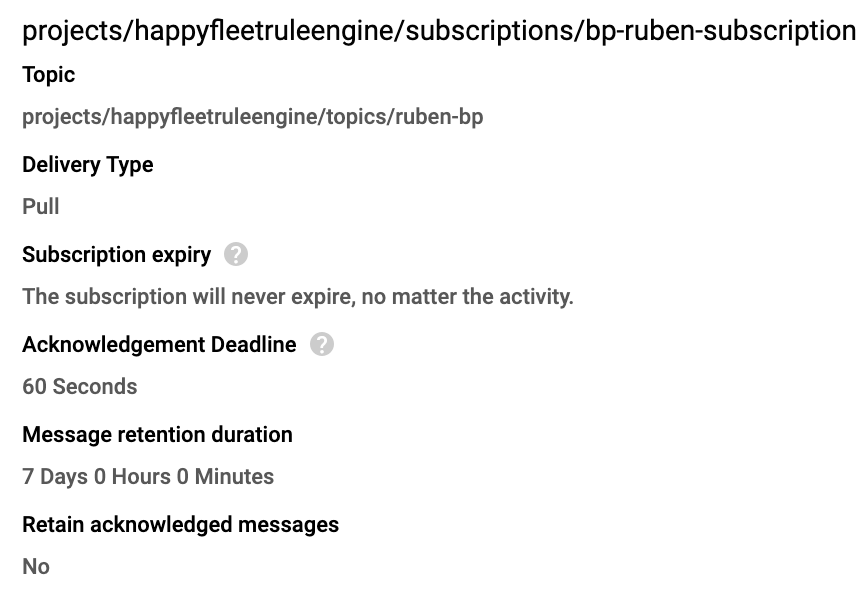
\includegraphics[width=140mm]{../gpsConfig.png}
    \caption{Configuratie van de topic voor de gebruikte subscription}
    
\end{figure}
\subsubsection{GooglePubSubConfig}
Zo ziet de GooglePubSubConfig.class eruit. Er worden twee kanalen aangemaakt van het type MessageChannel. Deze kanalen worden gebruikt om een bericht van een topic te lezen of verzenden.
        \begin{lstlisting}[language = Java , frame = trBL , firstnumber = last , escapeinside={(*@}{@*)}]
@Configuration
public class GooglePubSubConfig {
    @Bean("bachelorproef-channel-input")
    public MessageChannel createDeviceEventChannelInput() {
        return new DirectChannel();
    }
    
    @Bean("bachelorproef-channel-output")
    public MessageChannel createDeviceEventChannelOutput() {
        return new DirectChannel();
    }
    
    @Bean
    public PubSubInboundChannelAdapter createDeviceChannelAdapter(
    PubSubOperations pubSubTemplate,
    @Value("${pubsub.subscription}") String subsciptionName,
    @Qualifier("bachelorproef-channel-input") MessageChannel inputChannel,
    @Value("${pubsub.autostartup}") Boolean autoStart) {
        
        final PubSubInboundChannelAdapter adapter = new PubSubInboundChannelAdapter(pubSubTemplate, subsciptionName);
        adapter.setOutputChannel(inputChannel);
        adapter.setAckMode(AckMode.AUTO);
        adapter.setPayloadType(Event.class);
        adapter.setAutoStartup(autoStart);
        return adapter;
    }
    
    @Bean
    @ServiceActivator(inputChannel = "bachelorproef-channel-output")
    public MessageHandler messageSender(
    PubSubOperations pubsubTemplate,
    @Value("${pubsub.topic}") String topicName
    ) {
        return new PubSubMessageHandler(pubsubTemplate, topicName);
    }
    
    @Bean
    public JacksonPubSubMessageConverter createJacksonMessageConverter(final ObjectMapper objectMapper) {
        return new JacksonPubSubMessageConverter(objectMapper);
    }
    
}
     \end{lstlisting}
\subsubsection{GooglePubSubPublisher}
Deze klasse heeft maar één methode, namelijk publishData. Deze methode verstuurd het Data-object naar de topic via het kanaal \emph{bachelorproef-channel-output}. Er hoeft geen implementatie te zijn van deze methode, het spring-framework regelt al het andere werk in jouw plaats.
        \begin{lstlisting}[language = Java , frame = trBL , firstnumber = last , escapeinside={(*@}{@*)}]
@MessagingGateway(defaultRequestChannel = "bachelorproef-channel-output")
@Component
public interface GooglePubSubPublisher {
    void publishData(Data data);
    
}
     \end{lstlisting}
     
\section{Consumer project}
\section{Onderzoek}

